%\VignetteIndexEntry{Introduction to the USGSHydroOpt package}
%\VignetteEngine{knitr::knitr}
%\VignetteDepends{}
%\VignetteSuggests{}
%\VignetteImports{reshape2}
%\VignettePackage{USGSHydroOpt}

\documentclass[a4paper,11pt]{article}\usepackage[]{graphicx}\usepackage[]{color}
%% maxwidth is the original width if it is less than linewidth
%% otherwise use linewidth (to make sure the graphics do not exceed the margin)
\makeatletter
\def\maxwidth{ %
  \ifdim\Gin@nat@width>\linewidth
    \linewidth
  \else
    \Gin@nat@width
  \fi
}
\makeatother

\definecolor{fgcolor}{rgb}{0.345, 0.345, 0.345}
\newcommand{\hlnum}[1]{\textcolor[rgb]{0.686,0.059,0.569}{#1}}%
\newcommand{\hlstr}[1]{\textcolor[rgb]{0.192,0.494,0.8}{#1}}%
\newcommand{\hlcom}[1]{\textcolor[rgb]{0.678,0.584,0.686}{\textit{#1}}}%
\newcommand{\hlopt}[1]{\textcolor[rgb]{0,0,0}{#1}}%
\newcommand{\hlstd}[1]{\textcolor[rgb]{0.345,0.345,0.345}{#1}}%
\newcommand{\hlkwa}[1]{\textcolor[rgb]{0.161,0.373,0.58}{\textbf{#1}}}%
\newcommand{\hlkwb}[1]{\textcolor[rgb]{0.69,0.353,0.396}{#1}}%
\newcommand{\hlkwc}[1]{\textcolor[rgb]{0.333,0.667,0.333}{#1}}%
\newcommand{\hlkwd}[1]{\textcolor[rgb]{0.737,0.353,0.396}{\textbf{#1}}}%

\usepackage{framed}
\makeatletter
\newenvironment{kframe}{%
 \def\at@end@of@kframe{}%
 \ifinner\ifhmode%
  \def\at@end@of@kframe{\end{minipage}}%
  \begin{minipage}{\columnwidth}%
 \fi\fi%
 \def\FrameCommand##1{\hskip\@totalleftmargin \hskip-\fboxsep
 \colorbox{shadecolor}{##1}\hskip-\fboxsep
     % There is no \\@totalrightmargin, so:
     \hskip-\linewidth \hskip-\@totalleftmargin \hskip\columnwidth}%
 \MakeFramed {\advance\hsize-\width
   \@totalleftmargin\z@ \linewidth\hsize
   \@setminipage}}%
 {\par\unskip\endMakeFramed%
 \at@end@of@kframe}
\makeatother

\definecolor{shadecolor}{rgb}{.97, .97, .97}
\definecolor{messagecolor}{rgb}{0, 0, 0}
\definecolor{warningcolor}{rgb}{1, 0, 1}
\definecolor{errorcolor}{rgb}{1, 0, 0}
\newenvironment{knitrout}{}{} % an empty environment to be redefined in TeX

\usepackage{alltt}
\usepackage{amsmath}
\usepackage{times}
\usepackage{hyperref}
\usepackage[numbers, round]{natbib}
\usepackage[american]{babel}
\usepackage{authblk}
\usepackage{subfig}
\usepackage{placeins}
\usepackage{footnote}
\usepackage{tabularx}
\usepackage{parskip}
\usepackage{threeparttable}
\renewcommand\Affilfont{\itshape\small}

\renewcommand{\topfraction}{0.85}
\renewcommand{\textfraction}{0.1}
\usepackage{graphicx}

\textwidth=6.5in
\textheight=9.2in
\parskip=.3cm
\oddsidemargin=.1in
\evensidemargin=.1in
\headheight=-.3in

%------------------------------------------------------------
% newcommand
%------------------------------------------------------------
\newcommand{\scscst}{\scriptscriptstyle}
\newcommand{\scst}{\scriptstyle}
\newcommand{\Robject}[1]{{\texttt{#1}}}
\newcommand{\Rfunction}[1]{{\texttt{#1}}}
\newcommand{\Rclass}[1]{\textit{#1}}
\newcommand{\Rpackage}[1]{\textit{#1}}
\newcommand{\Rexpression}[1]{\texttt{#1}}
\newcommand{\Rmethod}[1]{{\texttt{#1}}}
\newcommand{\Rfunarg}[1]{{\texttt{#1}}}
\IfFileExists{upquote.sty}{\usepackage{upquote}}{}
\begin{document}






%------------------------------------------------------------
\title{USGSHydroOpt : Tools for Optical Analysis of Water}
%------------------------------------------------------------
\author[1]{Samuel Christel}
\author[1]{Steve Corsi}
\affil[1]{United States Geological Survey}




\maketitle
\tableofcontents

%------------------------------------------------------------
\section{Introduction to USGSHydroOpt}
%------------------------------------------------------------ 
The USGSHydroOpt package was created to streamline the process of creating optical summary variables and excitation-emission (EEMs) plots for absorbance and fluoresence data collected from various freshwater sources. Examples of optical summary variables that can be produced with this package include various absorbance peaks, The functions in this package were designed to operate on dataframes with a standard data structures. This package is not amenable to dataframes or arrays that do not fit the prescribed formats. The example dataframes and array in this package illustrate exactly how data structures should be formatted, and the examples illustrate how the functions operate on the data structures. Depicted below is an example of an EEMs plot produced with this package. The user is encouraged to step through each piece of R code as it is introduced in this document. In many instances a sample of the function output is provided (plots, tables), but not in all cases.

\begin{knitrout}
\definecolor{shadecolor}{rgb}{0.969, 0.969, 0.969}\color{fgcolor}
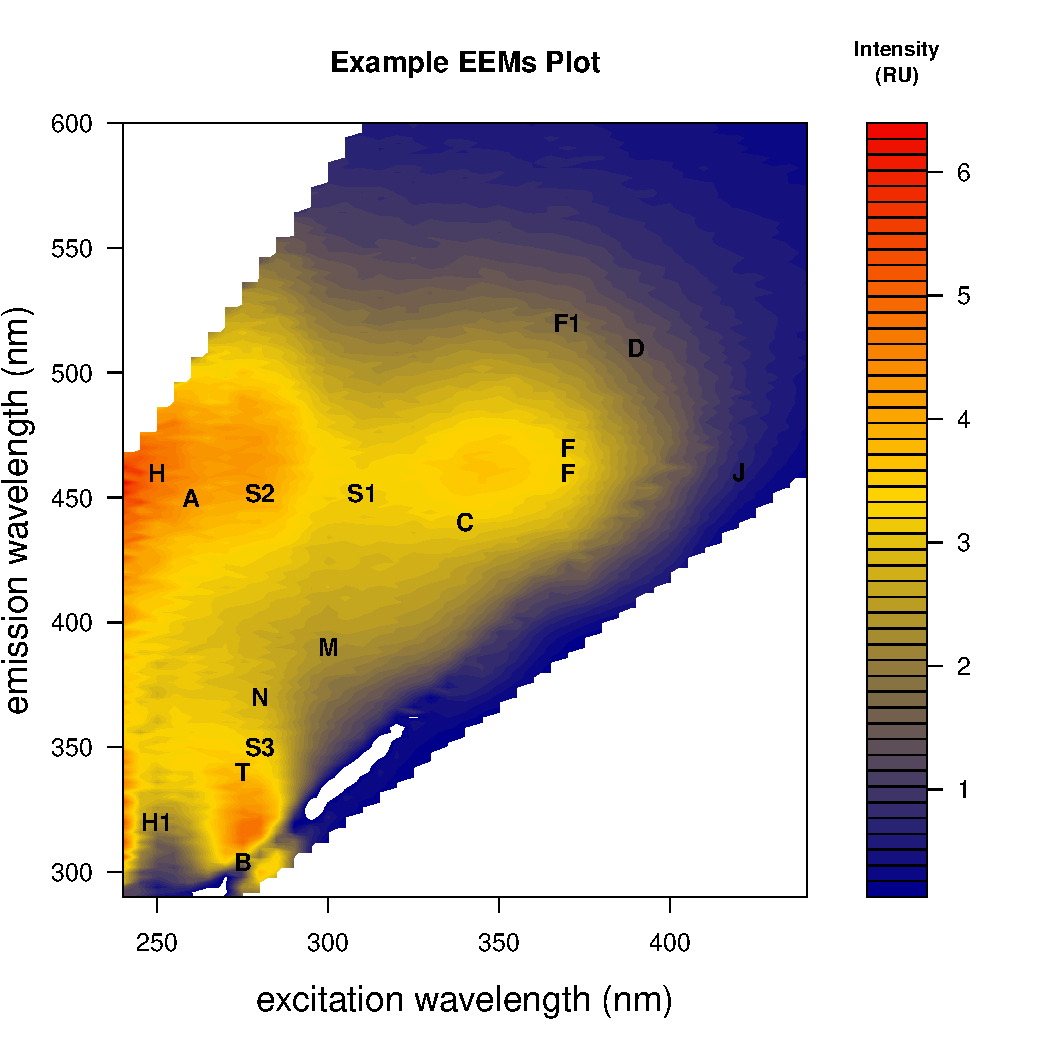
\includegraphics[width=\maxwidth]{figure/unnamed-chunk-3} 

\end{knitrout}

%------------------------------------------------------------
\section{Required Data Formats}
%------------------------------------------------------------ 
The functions contained in USGSHydroOpt operate on dataframes with defined structures. Users interested in using USGSHydroOpt should format dataframes according to the structures defined in this section.

%------------------------------------------------------------
\subsection{Absorbance Data}
%------------------------------------------------------------
Absorbance data used by functions in USGSHydroOpt should be formatted such that each sample occupies a column, and one column contains the wavelength (nm) for which the absorbance measurement was measured (\emph{See example Table 2.1 below}). The column with the wavelengths in Table 2.1 does not need to be called "wavelengths," as it is named in the example dataframe below. Since this package was developed primarily for USGS activities, the default for naming samples is "gr" then the sample number. This convention was started by the USGS California Water Sciences Center (CA WSC) and the USGS Wisconsin Water Science Center (WI WSC) follows the same naming convention to ensure standardization.

\begin{knitrout}
\definecolor{shadecolor}{rgb}{0.969, 0.969, 0.969}\color{fgcolor}\begin{kframe}
\begin{verbatim}
     gr13307    gr13351    gr13353    gr13357 wavelengths
1  0.0001296 -0.0003505 -0.0003480 -0.0002695         750
2 -0.0002367  0.0000305 -0.0000915 -0.0001407         749
3 -0.0001582 -0.0004900 -0.0006325 -0.0001534         748
4 -0.0004642 -0.0000105 -0.0000932 -0.0000245         747
5 -0.0002551 -0.0000653  0.0000841 -0.0001615         746
6 -0.0001842 -0.0002135  0.0002082  0.0001429         745
\end{verbatim}
\end{kframe}
\end{knitrout}

%------------------------------------------------------------
\subsection{Fluoresence Data}
%------------------------------------------------------------
Fluoresence data used by functions in USGSHydroOpt should also be formatted such that each sample occupies a column, and one column contains the excitation emission wavelength pairs (nm) for which the fluoresence measurment was measured (\emph{See example Table 2.2 below}). The column with the excitation emission pairs in Table 2.2 does not need to be called "Wavelength.Pairs," as it is in the example dataframe below. Again since this package was developed for USGS activities, the default sample naming convention is "gr" followed by the sample number.

\begin{knitrout}
\definecolor{shadecolor}{rgb}{0.969, 0.969, 0.969}\color{fgcolor}\begin{kframe}
\begin{verbatim}
  Wavelength.Pairs gr13307 gr13308  gr13351  gr13352
1          240/290 0.09457 0.05358 -0.07268 -0.19368
2          240/292 0.07386 0.09194  0.45433  0.39722
3          240/294 0.08116 0.09930  0.49135  0.37943
4          240/296 0.12013 0.09138 -0.12248  0.09239
5          240/298 0.15264 0.15428  0.54694  0.14980
6          240/300 0.16467 0.13010  0.43319  0.33064
\end{verbatim}
\end{kframe}
\end{knitrout}

%------------------------------------------------------------
\subsection{Spectral Slopes Data}
%------------------------------------------------------------
Information on the upper and lower wavelength (nm) for which a spectral slope should be calculated needs to be stored in a dataframe if USGSHydroOpt is used. The dataframe should contain exactly three columns. The first column should contain the upper wavelength, the second column should contain the lower wavelength, and the third column should contain the name of the spectral slope being calculated (\emph{See example Table 2.3 below}). The columns in Table 2.3 need to be in this exact order, although the names of the columns may be different. The data types for each column are integer, integer, and character, respectively. More spectral slopes can be added to the table than specified in the example dataframe below.

\begin{knitrout}
\definecolor{shadecolor}{rgb}{0.969, 0.969, 0.969}\color{fgcolor}\begin{kframe}
\begin{verbatim}
  wvlngth1 wvlngth2       Name
1      275      290 Sag275_295
2      290      350 Sag290_350
3      350      400 Sag350_400
4      412      676 Sag412_676
\end{verbatim}
\end{kframe}
\end{knitrout}

%------------------------------------------------------------
\subsection{Optical Summary Data}
%------------------------------------------------------------
This is the dataframe that contains many of the summary optical variables that can be produced using functions in USGSHydroOpt (\emph{See example Table 2.4a below}). The functions in USGSHydroOpt calculate summary optical variables and add to a dataframe formatted according to Table 2.4a below.  The example dataframe below is how the WI WSC stores optical summary variables. Note that this dataframe can contain other columns with metadata, for example, the sample data and time, the sample ID, or whether or not the sample went through QA/QC.

\begin{knitrout}
\definecolor{shadecolor}{rgb}{0.969, 0.969, 0.969}\color{fgcolor}\begin{kframe}
\begin{verbatim}
  GRnumber         B      T      A       J FI_2005    A254
1  gr13307  0.050997 0.1826 0.4553 0.03705   1.639 0.05228
2  gr13351 -0.245602 0.4085 3.0783 0.19110   1.456 0.43531
3  gr13353 -0.175220 0.7794 6.8624 0.56309   1.523 0.68274
4  gr13357  0.111561 0.2691 0.9451 0.06969   1.572 0.08698
5  gr13360 -0.001569 0.4593 2.8254 0.37231   1.563 0.28605
6  gr13363  0.052137 0.4892 1.9518 0.19098   1.583 0.19283
\end{verbatim}
\end{kframe}
\end{knitrout}

However, also note that summary optical variable names in the dataframe must be identical to those specified in Table 2.4b below. 

\begin{knitrout}
\definecolor{shadecolor}{rgb}{0.969, 0.969, 0.969}\color{fgcolor}\begin{kframe}
\begin{verbatim}
 [1] "OB1"        "OB2"        "OB3"        "S1.50"     
 [5] "S2.50"      "S3.50"      "S1.25"      "S2.25"     
 [9] "S3.25"      "Mrange.25"  "Mrange.50"  "B"         
[13] "T"          "M"          "A"          "C"         
[17] "N"          "D"          "F"          "J"         
[21] "S1"         "S2"         "S3"         "H1"        
[25] "H2"         "F1"         "F2"         "W"         
[29] "LT1"        "LT2"        "LT3"        "LA"        
[33] "HIX_2002"   "FI_2005"    "FI_2001"    "FreshI"    
[37] "A254"       "A275"       "A280"       "A290"      
[41] "A295"       "A350"       "A370"       "A400"      
[45] "A412"       "A440"       "A488"       "A510"      
[49] "A532"       "A555"       "A650"       "A676"      
[53] "A715"       "Sag275_290" "Sag290_350" "Sag350_400"
[57] "Sag412_676" "Aresids"   
\end{verbatim}
\end{kframe}
\end{knitrout}

%------------------------------------------------------------
\subsection{Excitation-Emission (EEMs) Peak Data}
%------------------------------------------------------------
The EEMs peak data contains three columns listing the name of a characterized EEM peak along with the corresponding wavelengths (nm) (\emph{See example Table 2.5 below}). The first column, in Table 2.5, "Peak," contains the name of the characterized EEM peak. The next two columns in Table 2.5 contain the excitation and emission wavelengths (nm) at which a given peak occurs. The column names must be identical to those displayed in the example below, although the order of the columns can be different. 

\begin{knitrout}
\definecolor{shadecolor}{rgb}{0.969, 0.969, 0.969}\color{fgcolor}\begin{kframe}
\begin{verbatim}
   Peak ExCA EmCA
1     B  275  304
2     T  275  340
3     M  300  390
4     A  260  450
5     C  340  440
6     N  280  370
7     D  390  510
8     F  370  460
9     J  420  460
10   S1  310  452
11   S2  280  452
12   S3  280  350
13    H  250  460
14   H1  250  320
15    F  370  470
16   F1  370  520
\end{verbatim}
\end{kframe}
\end{knitrout}

%------------------------------------------------------------
\subsection{Optical Ratio and Signals Data}
%------------------------------------------------------------
This dataframe contains one column called "ratioSignals" that contains all of the summary optical variables currently identified by the WI WSC (\emph{See example Table 2.6 below}). Note that these are the same variables as those listed in Table 2.4b. The first column must contain the various "ratioSignals" that the user desires, although the column name need not be "ratioSignals"

\begin{knitrout}
\definecolor{shadecolor}{rgb}{0.969, 0.969, 0.969}\color{fgcolor}\begin{kframe}
\begin{verbatim}
   ratioSignals keep
1           OB1   NA
2           OB2   NA
3           OB3   NA
4         S1.50   NA
5         S2.50   NA
6         S3.50   NA
7         S1.25   NA
8         S2.25   NA
9         S3.25   NA
10    Mrange.25   NA
11    Mrange.50   NA
12            B   NA
13            T   NA
14            M   NA
15            A   NA
16            C   NA
17            N   NA
18            D   NA
19            F   NA
20            J   NA
21           S1   NA
22           S2   NA
23           S3   NA
24           H1   NA
25           H2   NA
26           F1   NA
27           F2   NA
28            W   NA
29          LT1   NA
30          LT2   NA
31          LT3   NA
32           LA   NA
33     HIX_2002   NA
34      FI_2005   NA
35      FI_2001   NA
36       FreshI   NA
37         A254    1
38         A275    1
39         A280    1
40         A290    1
41         A295    1
42         A350    1
43         A370    1
44         A400    1
45         A412   NA
46         A440   NA
47         A488   NA
48         A510   NA
49         A532   NA
50         A555   NA
51         A650   NA
52         A676   NA
53         A715   NA
54   Sag275_290    1
55   Sag290_350    1
56   Sag350_400    1
57   Sag412_676    1
58      Aresids   NA
\end{verbatim}
\end{kframe}
\end{knitrout}

%------------------------------------------------------------
\subsection{Optical Signals Data}
%------------------------------------------------------------
This dataframe is similar to "ratioSignals" except it provides more metadata about peaks characterized for EEMs plots. The dataframe should contain six columns (\emph{See example Table 2.7 below}). The first column in Table 2.7, "Peak," contains the name of the characterized EEM peak. The next two columns, "Ex1" and "Ex2," contain the excitation wavelength range (nm) for a given peak. "Ex1" is the lower wavelength and "Ex2" is the upper wavelength for the excitation wavelength range (nm) for a given peak. Similarily, "Em1" and "Em2" contain the emission wavelength range (nm) for a given peak. The final column, "Source," lists the source that characterized the peak. The last column, "Source," is not required. The user must exactly replicate the column names in Table 2.7 in order for the code in USGSHydroOpt to run.

\begin{knitrout}
\definecolor{shadecolor}{rgb}{0.969, 0.969, 0.969}\color{fgcolor}\begin{kframe}
\begin{verbatim}
        Peak Ex1 Ex2 Em1 Em2                  Source
1        OB1 360  NA 410 598           Hartel Turner
2        OB2 360  NA 436 436           Hartel Turner
3        OB3 365  NA 400 550         Hagedorn Turner
4      S1.50 310  NA 402 502                 Sniffer
5      S2.50 280  NA 402 502                 Sniffer
6      S3.50 280  NA 310 390                 Sniffer
7      S1.25 310  NA 427 477                 Sniffer
8      S2.25 280  NA 427 477                 Sniffer
9      S3.25 280  NA 330 370                 Sniffer
10 Mrange.25 300  NA 365 415                    test
11 Mrange.50 300  NA 340 440                    test
12         B 275  NA 304  NA                      CA
13         T 275  NA 340  NA                      CA
14         M 300  NA 390  NA                      CA
15         A 260  NA 450  NA                      CA
16         C 340  NA 440  NA                      CA
17         N 280  NA 370  NA                      CA
18         D 390  NA 510  NA                      CA
19         F 370  NA 460  NA                      CA
20         J 420  NA 460  NA                      CA
21        S1 310  NA 452  NA                      CA
22        S2 280  NA 452  NA                      CA
23        S3 280  NA 350  NA                      CA
24        H1 250  NA 460  NA                Ohno2002
25        H2 250  NA 320  NA                Ohno2002
26        F1 370  NA 470  NA Cory and McKnight, 2005
27        F2 370  NA 520  NA Cory and McKnight, 2005
28         W 255 290 302 350                        
29       LT1 250  NA 340  NA                        
30       LT2 260  NA 340  NA                        
31       LT3 240  NA 340  NA                        
32        LA 240  NA 440  NA                        
\end{verbatim}
\end{kframe}
\end{knitrout}

%------------------------------------------------------------
\subsection{3-Dimensional Excitation-Emission Array}
%------------------------------------------------------------
A 3-D array with fluoresence data is used by many of the functions in USGSHydroOpt. The first dimension contains the excitation wavelengths (nm) as data type character at which a given fluoresence measurement was made. The second dimension contains the emission wavelengths (nm) as data type character at which a given fluoresence measurement was made. The third dimension contains the sample numbers as data type character for a given observation. The user must ensure that the third dimension of the array are sample numbers. Again, in this example the default "gr" followed by the sample number is used as a naming convention for samples.

To view the headers for each dimension using the following commands in R consider the example 3-D EEM array included with the USGSHydroOpt Package: 

\begin{knitrout}
\definecolor{shadecolor}{rgb}{0.969, 0.969, 0.969}\color{fgcolor}\begin{kframe}
\begin{alltt}
\hlcom{# this command shows the excitation wavelengths (nm)}
\hlkwd{colnames}\hlstd{(a)}
\end{alltt}
\begin{verbatim}
  [1] "290" "292" "294" "296" "298" "300" "302" "304" "306"
 [10] "308" "310" "312" "314" "316" "318" "320" "322" "324"
 [19] "326" "328" "330" "332" "334" "336" "338" "340" "342"
 [28] "344" "346" "348" "350" "352" "354" "356" "358" "360"
 [37] "362" "364" "366" "368" "370" "372" "374" "376" "378"
 [46] "380" "382" "384" "386" "388" "390" "392" "394" "396"
 [55] "398" "400" "402" "404" "406" "408" "410" "412" "414"
 [64] "416" "418" "420" "422" "424" "426" "428" "430" "432"
 [73] "434" "436" "438" "440" "442" "444" "446" "448" "450"
 [82] "452" "454" "456" "458" "460" "462" "464" "466" "468"
 [91] "470" "472" "474" "476" "478" "480" "482" "484" "486"
[100] "488" "490" "492" "494" "496" "498" "500" "502" "504"
[109] "506" "508" "510" "512" "514" "516" "518" "520" "522"
[118] "524" "526" "528" "530" "532" "534" "536" "538" "540"
[127] "542" "544" "546" "548" "550" "552" "554" "556" "558"
[136] "560" "562" "564" "566" "568" "570" "572" "574" "576"
[145] "578" "580" "582" "584" "586" "588" "590" "592" "594"
[154] "596" "598" "600"
\end{verbatim}
\begin{alltt}
\hlcom{# this command shows the emission wavelengths (nm)}
\hlkwd{rownames}\hlstd{(a)}
\end{alltt}
\begin{verbatim}
 [1] "240" "245" "250" "255" "260" "265" "270" "275" "280"
[10] "285" "290" "295" "300" "305" "310" "315" "320" "325"
[19] "330" "335" "340" "345" "350" "355" "360" "365" "370"
[28] "375" "380" "385" "390" "395" "400" "405" "410" "415"
[37] "420" "425" "430" "435" "440"
\end{verbatim}
\begin{alltt}
\hlcom{# this command shows the emission wavelengths (nm), only the}
\hlcom{# first 20 shown for simplicity}
\hlkwd{names}\hlstd{(a[}\hlnum{1}\hlstd{,} \hlnum{1}\hlstd{, ])[}\hlnum{1}\hlopt{:}\hlnum{20}\hlstd{]}
\end{alltt}
\begin{verbatim}
 [1] "gr13307" "gr13308" "gr13351" "gr13352" "gr13353"
 [6] "gr13354" "gr13357" "gr13358" "gr13360" "gr13361"
[11] "gr13362" "gr13363" "gr13364" "gr13365" "gr13374"
[16] "gr13375" "gr13433" "gr13434" "gr13435" "gr13439"
\end{verbatim}
\end{kframe}
\end{knitrout}

The user should be aware of \textbf{two important caveats}: (1) There should rarely be emission wavelengths below the excitation wavelength for a given fluoresence reading. Where this occurs an NA will be found in the 3-D EEMs array. (2) Intensities at an emission wavelength that is two times the excitation wavelength will be influence by second order Rayleigh scatter. 

%------------------------------------------------------------
\subsection{Creating a 3-Dimensional Excitation-Emission Array}
%------------------------------------------------------------
In Section 2.8 the format of 3-D arrays of fluoresence data that can be used with USGSHydroOpt was discussed. USGSHydroOpt can also be used to produce such arrays given the appropriate input fluoresence dataframe. Below is an example of how USGSHydroOpt is used to accomplish this task: 

\begin{knitrout}
\definecolor{shadecolor}{rgb}{0.969, 0.969, 0.969}\color{fgcolor}\begin{kframe}
\begin{alltt}
\hlcom{# set an arbitrary data frame (df) as dfFluor (the example}
\hlcom{# fluoresence dataframe in USGSHydroOpt)}
\hlstd{df} \hlkwb{<-} \hlstd{dfFluor}

\hlcom{# define the column in dfFluor}
\hlstd{ExEm} \hlkwb{<-} \hlstr{"Wavelength.Pairs"}

\hlcom{# run the VectorizedTo3DArray function from USGSHydroOpt that}
\hlcom{# creates a 3-D EEMs array given a vectorized fluoresence}
\hlcom{# dataframe}
\hlstd{aTest} \hlkwb{<-} \hlkwd{VectorizedTo3DArray}\hlstd{(df, ExEm)}
\end{alltt}
\end{kframe}
\end{knitrout}

In the example above, dfFluor is formatted according to the fluoresence dataframe discussed in Section 2.2. 

%------------------------------------------------------------
\section{Creating Summary Optical Variables}
%------------------------------------------------------------ 
Most of the functions included in USGSHydroOpt are for creating variables that summarize optical data. Such variables can then be used in statistical modeling efforts aimed at describing observed phenomena in aquatic ecosystems. This sections steps through the six functions that USGSHydroOpt offers for creating such summary optical variables.

%------------------------------------------------------------
\subsection{Creating Absorbance Coefficients}
%------------------------------------------------------------ 
The function getAbs opperates on a dataframe formatted according to Section 2.1. Specifically, it picks out absorbance coefficients for a defined set of wavelengths (nm) and adds those coefficients to an optical summary data frame formatted according to Section 2.4. Shown below is an example of how the function can be used.

\begin{knitrout}
\definecolor{shadecolor}{rgb}{0.969, 0.969, 0.969}\color{fgcolor}\begin{kframe}
\begin{alltt}
\hlcom{# assign a variable dataAbs to the absorbance dataframe}
\hlcom{# included in USGSHydroOpt}
\hlstd{dataAbs} \hlkwb{<-} \hlstd{dfabs}

\hlcom{# define the column with the wavelengths in dataAbs}
\hlstd{waveCol} \hlkwb{<-} \hlstr{"wavelengths"}

\hlcom{# define the wavelengths for which absorbance coefficients}
\hlcom{# should be defined}
\hlstd{wavs} \hlkwb{<-} \hlkwd{c}\hlstd{(}\hlnum{430}\hlstd{,} \hlnum{530}\hlstd{,} \hlnum{630}\hlstd{,} \hlnum{730}\hlstd{)}

\hlcom{# define which columns contain the absorbance data, by}
\hlcom{# default per WI WSC and CA WSC samples start with 'gr'}
\hlstd{colSubsetString} \hlkwb{<-} \hlstr{"gr"}

\hlcom{# assign a variable dataSummary to the dfsummary dataframe}
\hlcom{# included in USGSHydroOpt}
\hlstd{dataSummary} \hlkwb{<-} \hlstd{dfsummary}

\hlcom{# assign a variable grnum to the column in dataSummary with}
\hlcom{# sample numbers}
\hlstd{grnum} \hlkwb{<-} \hlstr{"GRnumber"}

\hlcom{# use getAbs to produce absorbance coefficients}
\hlstd{testAbs} \hlkwb{<-} \hlkwd{getAbs}\hlstd{(dataAbs, waveCol, wavs, colSubsetString, dataSummary,}
    \hlstd{grnum)}

\hlcom{# note that the absorbance coefficients as defined by wavs}
\hlcom{# have been added to dataSummary}
\hlkwd{colnames}\hlstd{(testAbs)[}\hlnum{69}\hlopt{:}\hlnum{72}\hlstd{]}
\end{alltt}
\begin{verbatim}
[1] "A430" "A530" "A630" "A730"
\end{verbatim}
\end{kframe}
\end{knitrout}

%------------------------------------------------------------
\subsection{Spectral Slopes by Linear Regression}
%------------------------------------------------------------ 
The function getExpResid computes spectral slopes by a first order decay function determined by linear regression (Helms et al. 2008).The residual at a specified wavelength (nm) is then calculated based on the spectral slope. The residual at a given wavelength and spectral slope is then added to a summary dataframe formatted according to Section 2.4. Displayed below is an example of how the function can be used. The function produces a plot with the absorbance data for each sample. On the plot the red indicates the spectral slope model, the blue is the absorbance data in rangeGap, and the black is the data in rangeReg but not in rangeGap. The dataframe dataAbs is formatted according to Section 2.1, but is shortened. If the user calls "pdf(genericName.pdf)," \emph{See }?pdf, then runs the function plots will be printed to the pdf in the working directory. 

\begin{knitrout}
\definecolor{shadecolor}{rgb}{0.969, 0.969, 0.969}\color{fgcolor}\begin{kframe}
\begin{alltt}
\hlcom{# absorbance wavelength (nm) for which residual is calculated}
\hlstd{wavelength} \hlkwb{<-} \hlnum{267}

\hlcom{# the absorbance wavelength range (nm) to be considered as a}
\hlcom{# numeric string}
\hlstd{rangeReg} \hlkwb{<-} \hlkwd{c}\hlstd{(}\hlnum{240}\hlstd{,} \hlnum{340}\hlstd{)}

\hlcom{# the absorbance wavelength range (nm) to be considered as a}
\hlcom{# numeric string}
\hlstd{rangeGap} \hlkwb{<-} \hlkwd{c}\hlstd{(}\hlnum{255}\hlstd{,} \hlnum{300}\hlstd{)}

\hlcom{# assign a variable dataAbs to a shortened version of the}
\hlcom{# absorbance dataframe included in USGSHydroOpt}
\hlstd{dataAbs} \hlkwb{<-} \hlstd{dfabs}

\hlcom{# define the column with the wavelengths in dataAbs}
\hlstd{waveCol} \hlkwb{<-} \hlstr{"wavelengths"}

\hlcom{# assign a variable grnum to the column in dataSummary with}
\hlcom{# sample numbers}
\hlstd{colSubsetString} \hlkwb{<-} \hlstr{"gr"}

\hlcom{# assign a variable dataSummary to the dfsummary dataframe}
\hlcom{# included in USGSHydroOpt, column 68 or 'Aresids' is removed}
\hlcom{# because we are computing this summary optical variable with}
\hlcom{# this function and then adding it to dataSummary}
\hlstd{dataSummary} \hlkwb{<-} \hlstd{dfsummary[,} \hlopt{-}\hlkwd{c}\hlstd{(}\hlnum{68}\hlstd{)]}

\hlcom{# assign a variable grnum to the column in dataSummary with}
\hlcom{# sample numbers}
\hlstd{grnum} \hlkwb{<-} \hlstr{"GRnumber"}

\hlcom{# use getExpResid to calculate the residual at a given}
\hlcom{# wavelength given a spectral slope calculated per Helms et}
\hlcom{# al. 2008.}
\hlstd{testdfOpt} \hlkwb{<-} \hlkwd{getExpResid}\hlstd{(wavelength, rangeReg, rangeGap, dataAbs,}
    \hlstd{waveCol, colSubsetString, dataSummary, grnum)}

\hlcom{# notice that the variable 'Aresids' has been added to}
\hlcom{# dataSummary}
\hlkwd{colnames}\hlstd{(testdfOpt)}
\end{alltt}
\end{kframe}
\end{knitrout}

The function  getSag blah blah blah


%------------------------------------------------------------
\subsection{Humification and Fluoresence Indices}
%------------------------------------------------------------ 
Four humification and fluoresence index summary variables can be computed using the function getIndexes. The the humification index summary variable called "HIX\textunderscore 2002" is calculated according to Ohno (2002). The first fluoresence index summary variable "FI\textunderscore 2005" is computed according to Cory and McKnight (2005). The second fluoresence index summary variable, "FI\textunderscore 2001" is computed according to McKnight et al. (2001). The final summary variable produced by this function is the freshness index, "FreshI," is computed according to Parlanti et al. (2000). Each of these four summary variables are computed and added to the optical summary dataframe, formatted according to Section 2.4. In the example below, getIndexes is used to compute the four summary variables, which are subsequently added to an optical summary dataframe. A 3-dimensional excitation-emission dataframe with fluoresence data formatted according to Sections 2.8-2.9 is used in computing these summary variables.

\begin{knitrout}
\definecolor{shadecolor}{rgb}{0.969, 0.969, 0.969}\color{fgcolor}\begin{kframe}
\begin{alltt}
\hlcom{# set a variable a as the example 3-D excitation emission}
\hlcom{# array included with the package}
\hlstd{a} \hlkwb{<-} \hlstd{a}

\hlcom{# assign a variable dataSummary to the dfsummary dataframe}
\hlcom{# included in USGSHydroOpt}
\hlstd{dataSummary} \hlkwb{<-} \hlstd{dfsummary}

\hlcom{# remove those columns with the fluoresence and humic indices}
\hlcom{# that we are computing here}
\hlstd{dataSummary} \hlkwb{<-} \hlstd{dataSummary[,} \hlopt{-}\hlkwd{c}\hlstd{(}\hlnum{43}\hlopt{:}\hlnum{46}\hlstd{)]}

\hlcom{# assign a variable grnum to the column in dataSummary with}
\hlcom{# sample numbers}
\hlstd{grnum} \hlkwb{<-} \hlstr{"GRnumber"}

\hlcom{# use getIndexes to compute the four humification and}
\hlcom{# fluoresence indices}
\hlstd{testIndexes} \hlkwb{<-} \hlkwd{getIndexes}\hlstd{(a, dataSummary, grnum)}

\hlcom{# note that the four indices have been added to dataSummary}
\hlkwd{colnames}\hlstd{(testIndexes)[}\hlnum{65}\hlopt{:}\hlnum{68}\hlstd{]}
\end{alltt}
\begin{verbatim}
[1] "HIX_2002" "FI_2005"  "FI_2001"  "FreshI"  
\end{verbatim}
\end{kframe}
\end{knitrout}

%------------------------------------------------------------
\subsection{Freshness Index}
%------------------------------------------------------------ 

%------------------------------------------------------------
\subsection{Optical Ratios}
%------------------------------------------------------------ 
The function getRatios uses absorbance peaks and spectral slopes in an existing summary optical data frame (e.g., dfsummary) and creates ratios between the different peaks and ratios. These ratios can be useful as predictor variables in statistical modeling efforts. In the example, below 65 different ratios are computed using an optical summary dataframe formatted per Section 2.4, and the ratioSignals example dataframe formatted per Section 2.6. The names of the calculated ratios added to the optical summary dataframe begin with "r" to signify "ratio" followed by the absorbance peak and/or spectral slope used to calculate the ratio. For example, the ratio of the absorbance peak at 254nm (A254) and the spectral slope between 350 and 400nm (Sag350\textunderscore 400) is called "rA254\textunderscore Sag350\textunderscore 400."


\begin{knitrout}
\definecolor{shadecolor}{rgb}{0.969, 0.969, 0.969}\color{fgcolor}\begin{kframe}
\begin{alltt}
\hlcom{# assign a variable dataSummary to the dfsummary dataframe}
\hlcom{# included in USGSHydroOpt}
\hlstd{dataSummary} \hlkwb{<-} \hlstd{dfsummary}

\hlcom{# note the number of variables in dataSummary}
\hlkwd{length}\hlstd{(}\hlkwd{colnames}\hlstd{(dataSummary))}
\end{alltt}
\begin{verbatim}
[1] 68
\end{verbatim}
\begin{alltt}
\hlcom{# pick out the absorbance peaks and spectral slopes to be}
\hlcom{# used for calculating ratios these correspond to those with}
\hlcom{# a 1 in the 'keep' column.}
\hlstd{sigs} \hlkwb{<-} \hlstd{ratioSignals[}\hlkwd{which}\hlstd{(ratioSignals[}\hlnum{2}\hlstd{]} \hlopt{>} \hlnum{0}\hlstd{),} \hlnum{1}\hlstd{]}

\hlcom{# assign a variable grnum to the column in dataSummary with}
\hlcom{# sample numbers}
\hlstd{grnum} \hlkwb{<-} \hlstr{"GRnumber"}

\hlcom{# use getRatios to calculate 65 different ratios of}
\hlcom{# absorbance peaks and spectral slopes}
\hlstd{test} \hlkwb{<-} \hlkwd{getRatios}\hlstd{(dataSummary, sigs, grnum)}

\hlcom{# notice that 65 ratios have been added to dataSummary}
\hlkwd{length}\hlstd{(}\hlkwd{colnames}\hlstd{(test))}
\end{alltt}
\begin{verbatim}
[1] 134
\end{verbatim}
\begin{alltt}
\hlcom{# example of some ratios added}
\hlkwd{colnames}\hlstd{(test)[}\hlnum{69}\hlopt{:}\hlnum{75}\hlstd{]}
\end{alltt}
\begin{verbatim}
[1] "rA254_A275" "rA254_A280" "rA254_A290" "rA254_A295"
[5] "rA254_A350" "rA254_A370" "rA254_A400"
\end{verbatim}
\end{kframe}
\end{knitrout}

%------------------------------------------------------------
\subsection{Log transformation of Summary Optical Variables}
%------------------------------------------------------------ 


\end{document}
